\chapter{Sample Extracts and Visualizations}
\label{app:sample_outputs}

This appendix provides raw excerpts of the serialization formats generated by the document intelligence pipeline, alongside visual validations of the detection models.

\section{Hierarchical Knowledge Graph (HKG) JSON Serialization}
The following is an excerpt from a generated \texttt{\_graph.json} manifest representing a strictly parsed industrial product specification. It demonstrates the structural breadcrumb context and nested Markdown payloads utilized for Retrieval-Augmented Generation.

\begin{lstlisting}[language=json]
{
    "doc_id": "7000-12121-2350400",
    "filename": "7000-12121-2350400.pdf",
    "nodes": [
        {
            "node_id": "node_001",
            "type": "text",
            "hierarchy": [
                "M12 male 90 deg  A-cod. with cable"
            ],
            "content": "[CONTEXT: M12 male 90 deg  A-cod.]\n\n## M12 male 90 deg  A-cod.",
            "metadata": {
                "node_type": "text",
                "contains_table": false,
                "contains_figure": false,
                "page": 1,
                "breadcrumb": "M12 male 90 deg  A-cod. with cable",
                "bbox": [39.71, 94.60, 183.92, 107.37]
            }
        },
        {
            "node_id": "node_008",
            "type": "table",
            "hierarchy": [
                "Link to Product"
            ],
            "content": "| Cable length | 4 m |\n| --- | --- |\n| Tightening torque | 0.6 Nm |",
            "metadata": {
                "node_type": "table",
                "contains_table": true,
                "breadcrumb": "Link to Product",
                "bbox": [39.16, 330.64, 555.98, 779.63]
            }
        }
    ]
}
\end{lstlisting}

\section{Bounding Box Visualizations}
To functionally validate the performance of DocLayout-YOLO against highly dense, unstructured layouts, bounding box visualization was employed. Figure \ref{fig:app_bbox} demonstrates a "Before and After" state mapping abstract PDF matrices to perfectly constrained bounding parameters.

\begin{figure}[htbp]
\centering
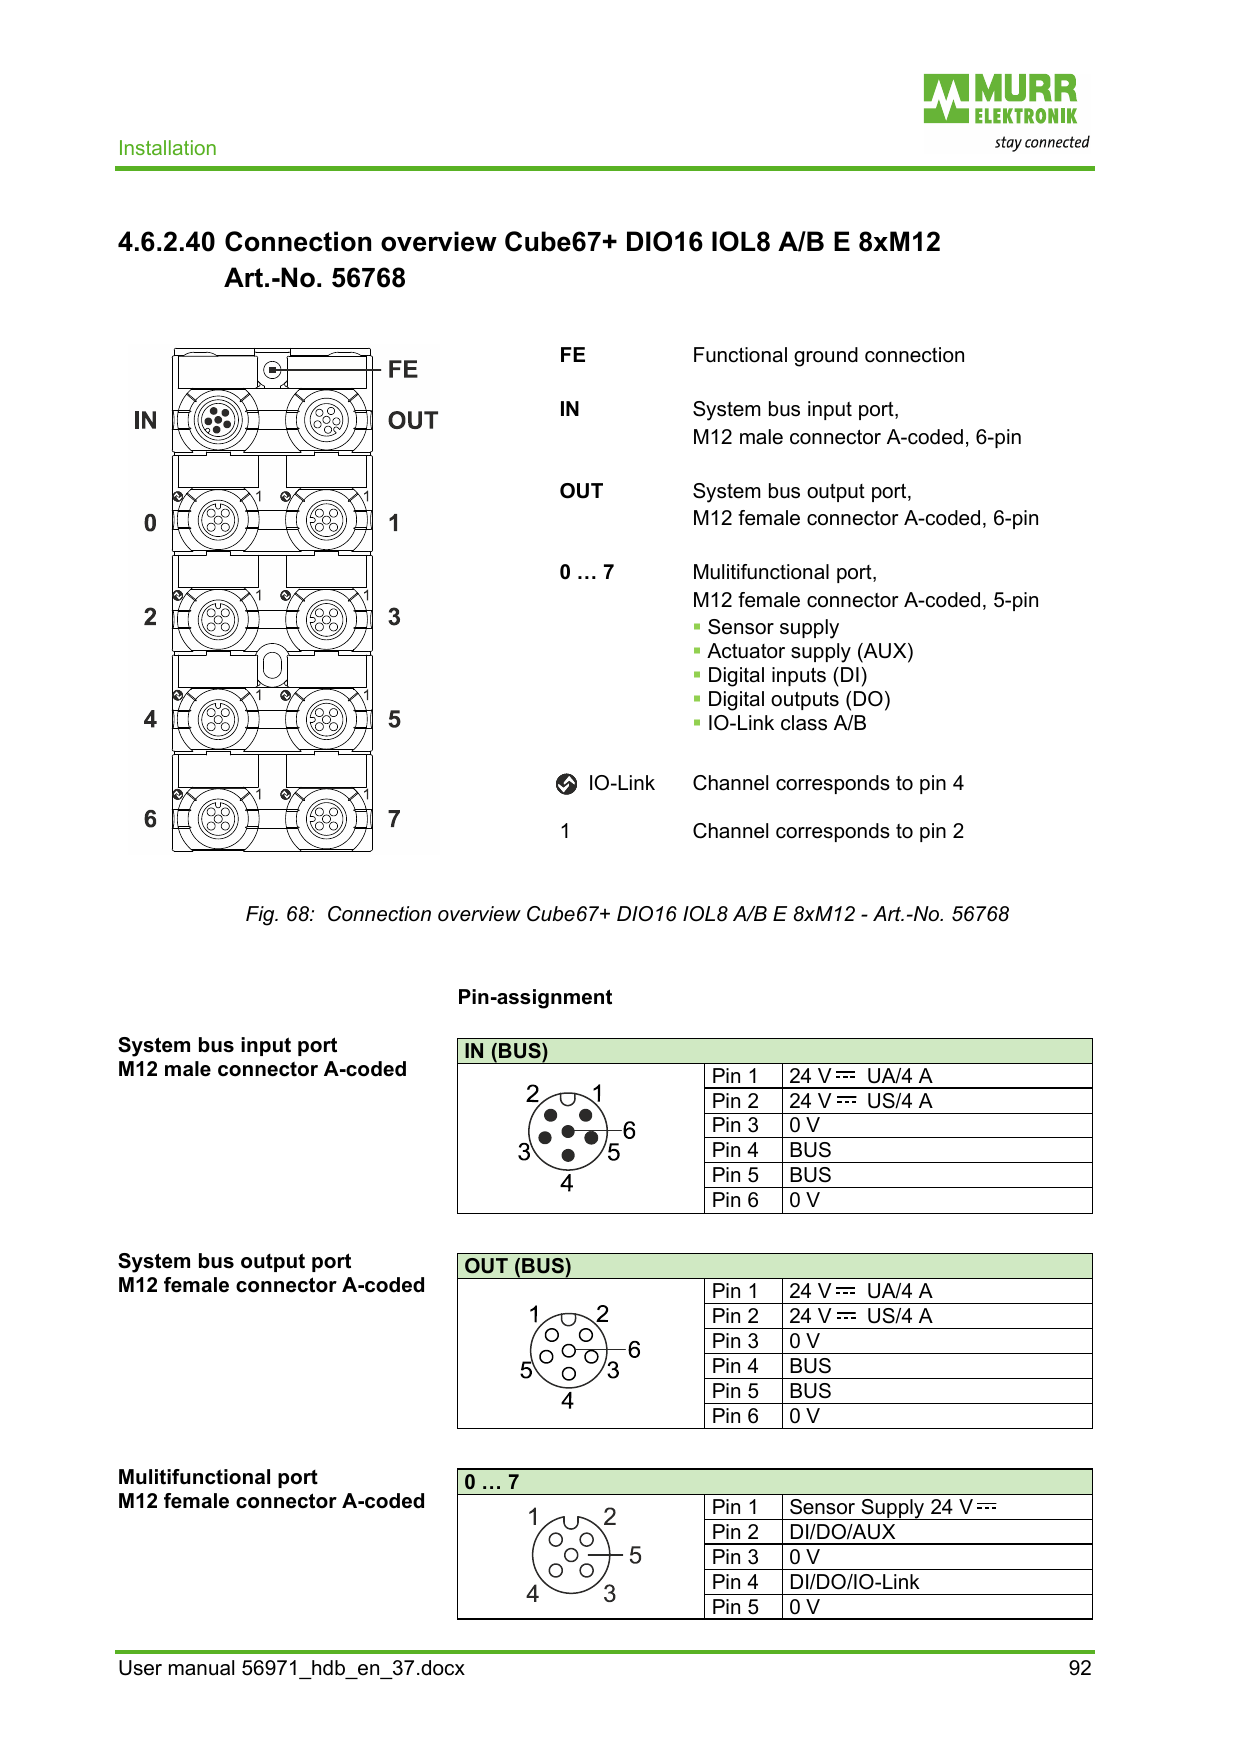
\includegraphics[width=0.48\textwidth]{images/Super_Complex_2-1.png}
\hfill
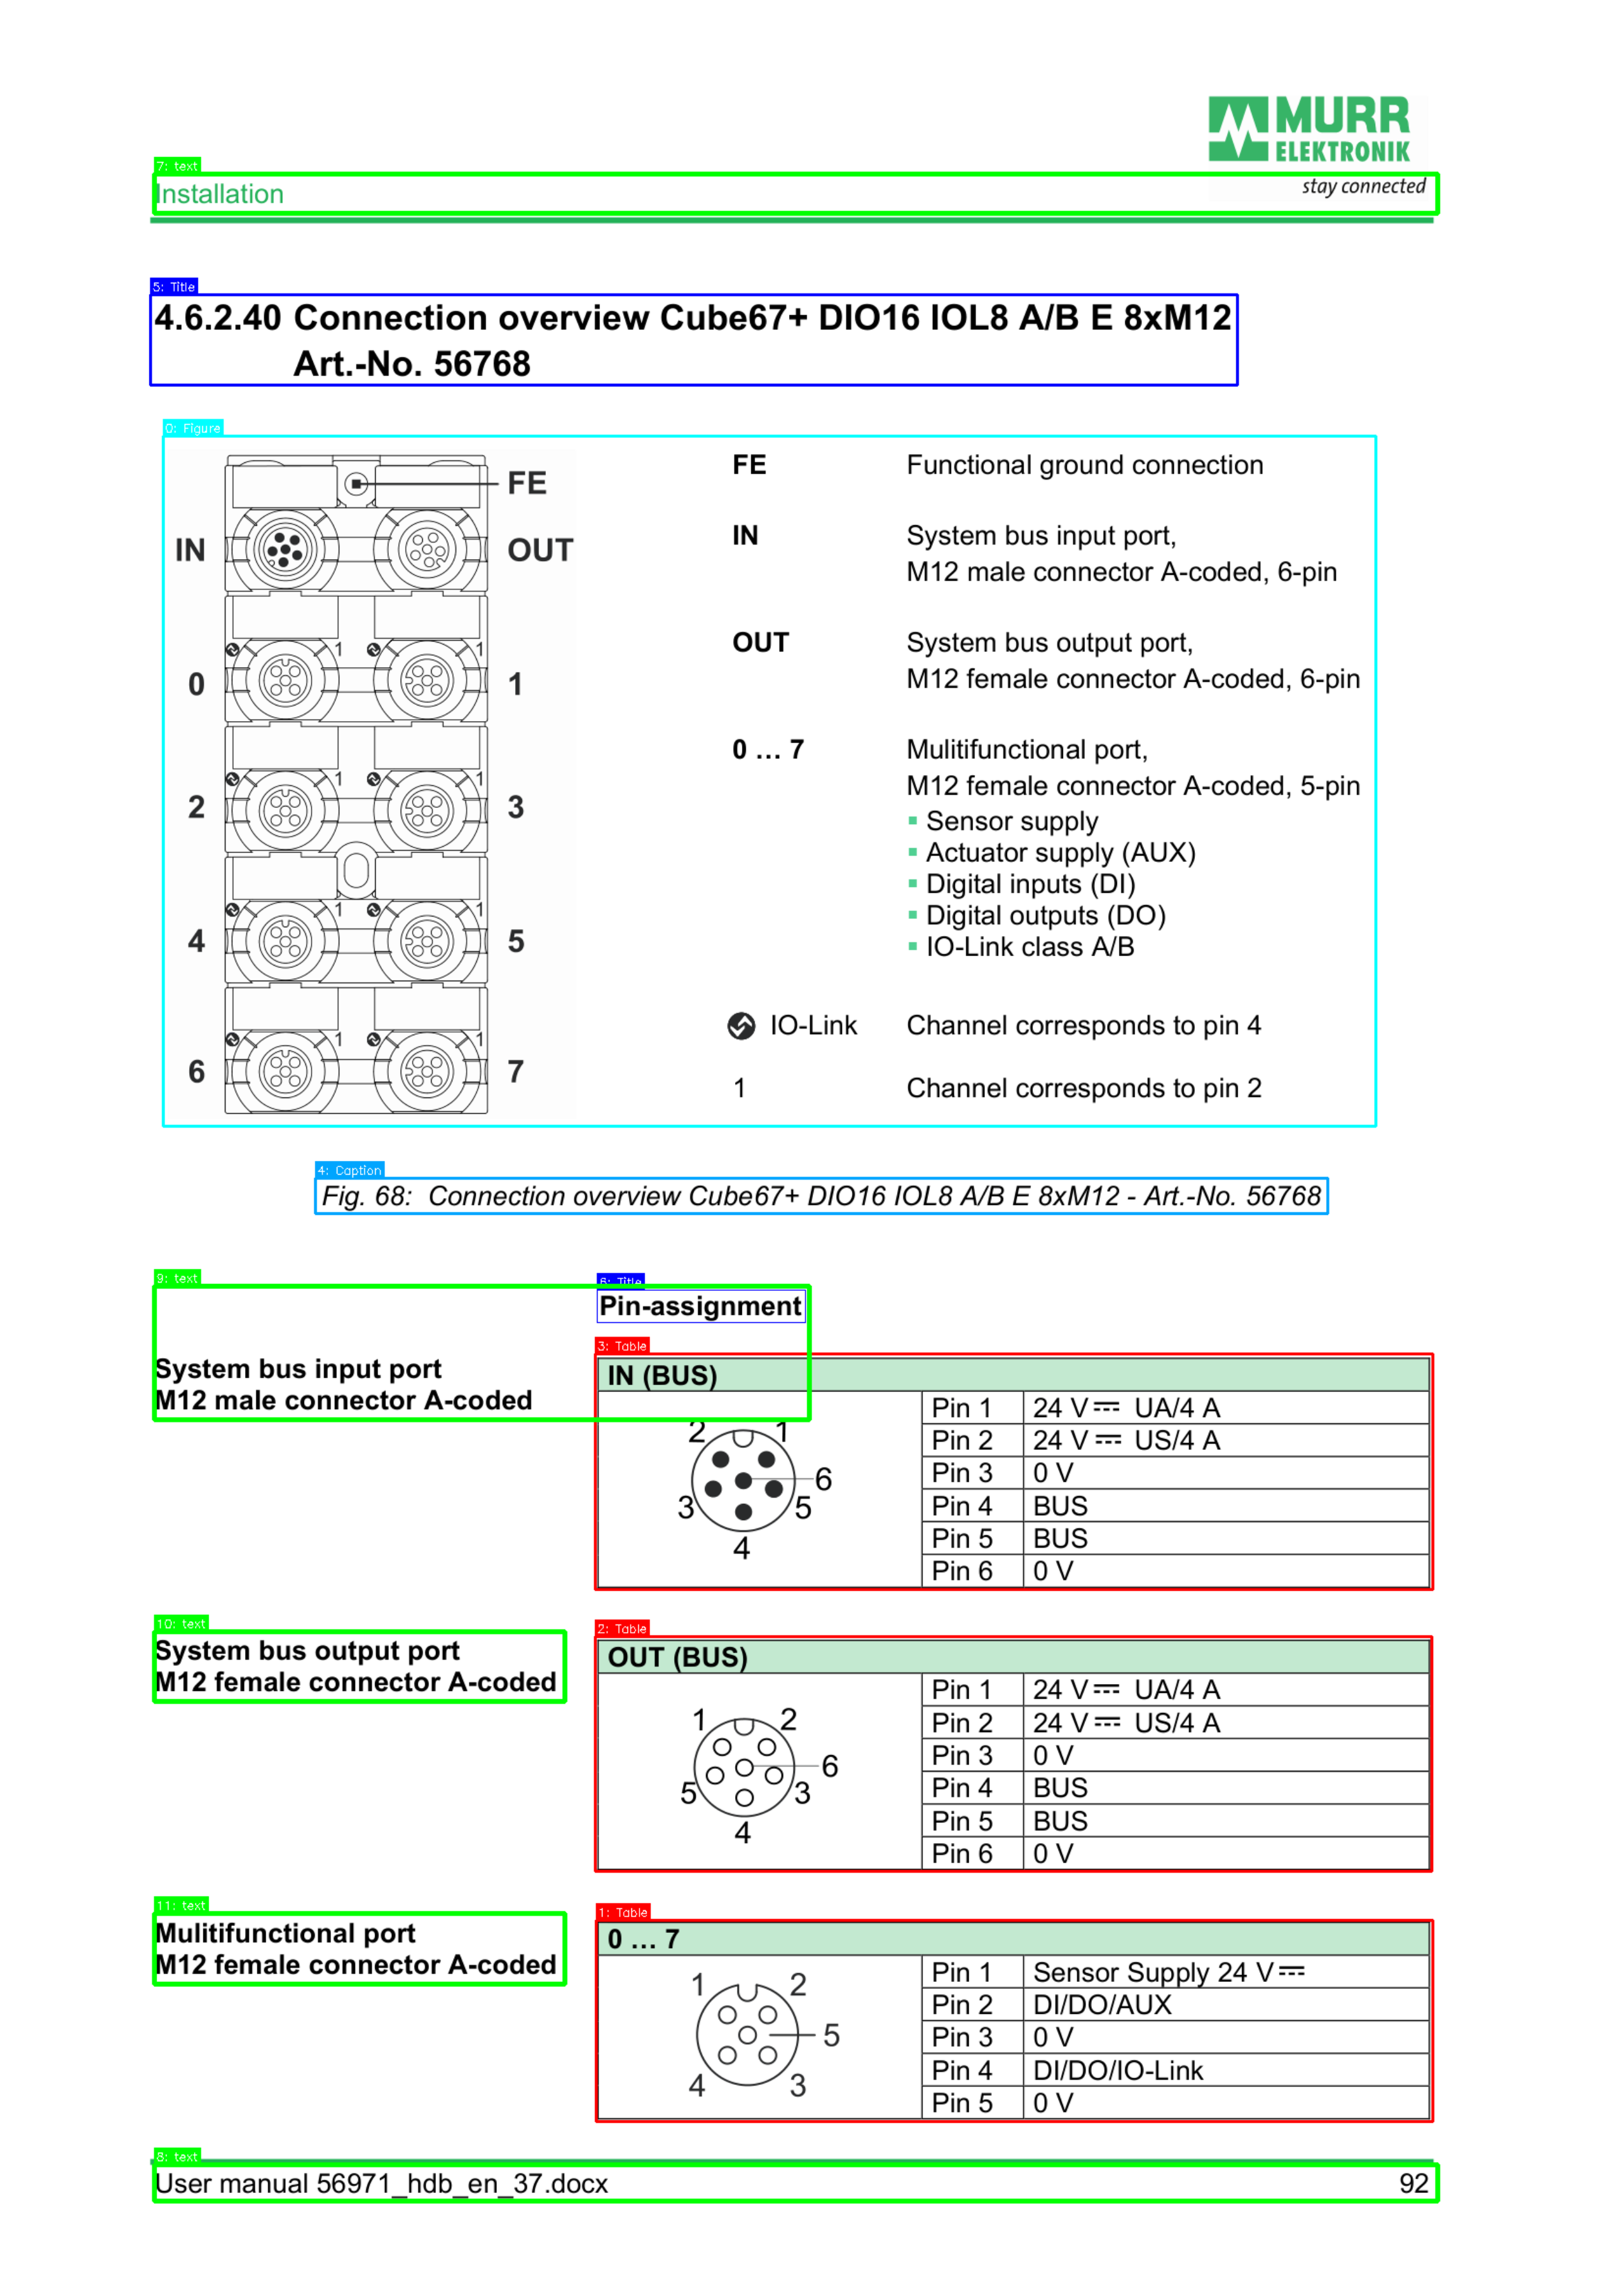
\includegraphics[width=0.48\textwidth]{images/layout_visualizations-1.png}
\caption{Visual layout detection applied to a dense engineering catalog. The system processes the raw structural PDF and maps the resulting YOLOv10 prediction tensors encapsulating the regions.}
\label{fig:app_bbox}
\end{figure}
